\section{lemma8}
\begin{lemma}
\end{lemma}

Suppose we have a Riemann sphere $C$ and a diagram $(C,\iota,\xi)$ and a regular cell complex refinement $\overline{(C,\iota,\xi)}$ and a sheaf $\mathfrak{F}$ singular supported on it such that when restricted to a small disk $D\subset C$, the refinement is as the following figure where two dimensional strata are labeled :

\begin{figure}[H] % Optional: [h] means here, [t] for top, [b] for bottom, [p] for page of floats
    \centering
    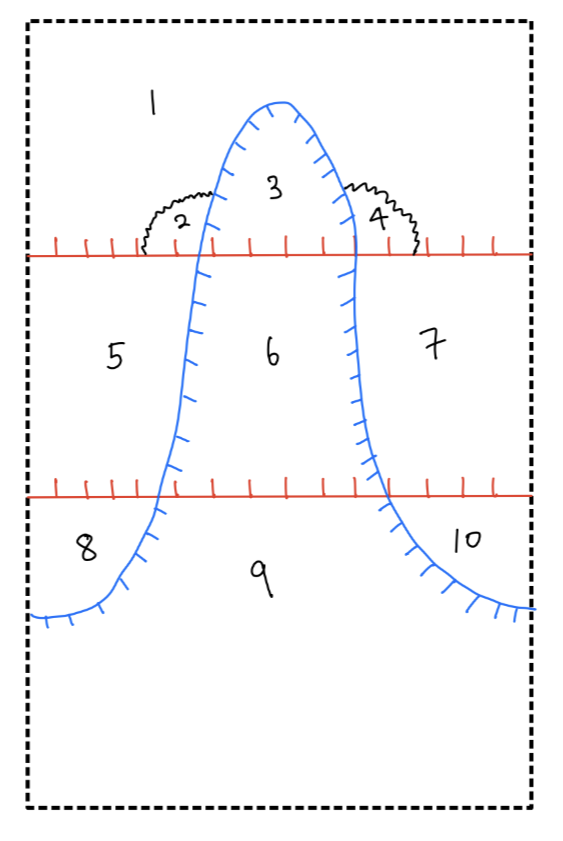
\includegraphics[width=\linewidth]{diagrams/lemma8/1.png} % Adjust the width as needed
    \caption{Your caption here}
    \label{fig:your-label}
\end{figure}

Stalks :\\
- 1 : $0$
- 2 : $\mathbb{C}\xrightarrow{\times a}\mathbb{C}$\\
- 3 : $\mathbb{C}[-1]$\\
- 4 : $\mathbb{C}\xrightarrow{\times b}\mathbb{C}$\\
- 5 : $\mathbb{C}$\\
- 6 : $0$\\
- 7 : $\mathbb{C}$\\
- 8 : $\mathbb{C}^2$\\
- 9 : $\mathbb{C}$\\
- 10 : $\mathbb{C}^2$\\

Generization maps :\\
I won't write down the zero maps.\\
- 3$\rightarrow$2 : 
\begin{tikzcd}
\mathbb{C} \arrow[r,"id"]     & \mathbb{C}  \\
0 \arrow[r,]\arrow[u,] & \mathbb{C} \arrow[u,"\times a"]
\end{tikzcd}
\\
- 3$\rightarrow$4 : 
\begin{tikzcd}
\mathbb{C} \arrow[r,"id"]     & \mathbb{C}  \\
0 \arrow[r,]\arrow[u,] & \mathbb{C} \arrow[u,"\times b"]
\end{tikzcd}
\\
- 2$\rightarrow$5 : 
\begin{tikzcd}
\mathbb{C} \arrow[r,]     & 0  \\
\mathbb{C} \arrow[r,"id"]\arrow[u,"\times a"] & \mathbb{C} \arrow[u,]
\end{tikzcd}
\\
- 4$\rightarrow$7 : 
\begin{tikzcd}
\mathbb{C} \arrow[r,]     & 0  \\
\mathbb{C} \arrow[r,"id"]\arrow[u,"\times b"] & \mathbb{C} \arrow[u,]
\end{tikzcd}
\\

- 5$\rightarrow$8 : $\iota_f$\\
- 9$\rightarrow$8 ,9$\rightarrow$10 : $\iota_l$\\
- 7$\rightarrow$10 : $\mathbb{C}\rightarrow \mathbb{C}^2$ where $1\mapsto (x,y)^T$ where $x\neq 0$\\

Now we will define isotopy starting from $\mathfrak{F}$ to the final sheaf $\mathfrak{F}'$ which is described as follows:\\

\begin{figure}[H] % Optional: [h] means here, [t] for top, [b] for bottom, [p] for page of floats
    \centering
    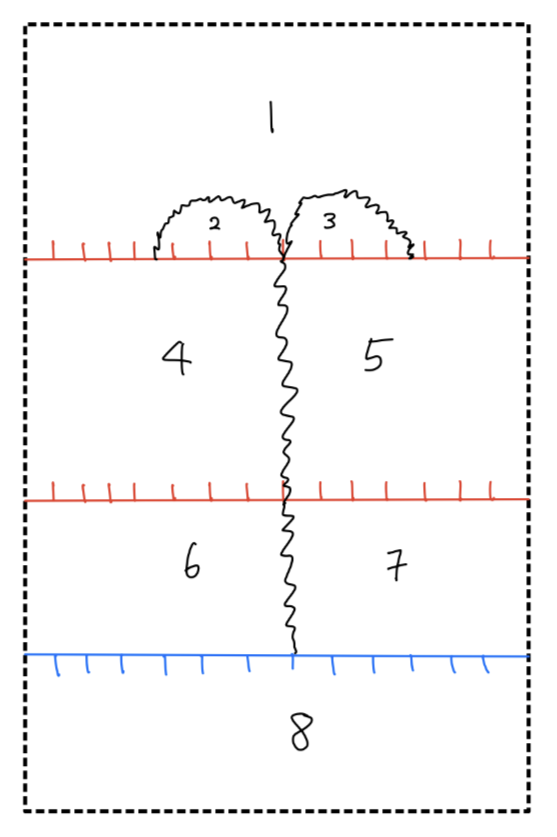
\includegraphics[width=\linewidth]{diagrams/lemma8/2.png} % Adjust the width as needed
    \caption{Your caption here}
    \label{fig:your-label}
\end{figure}

Stalks : \\
- 1: $0$\\
- 2 : $\mathbb{C}\xrightarrow{\times a}\mathbb{C}$\\
- 3 : $\mathbb{C}\xrightarrow{\times b}\mathbb{C}$\\
- 4 : $\mathbb{C}$\\
- 5 : $\mathbb{C}$\\
- 6 : $\mathbb{C}$\\
- 7 : $\mathbb{C}$\\
- 8 : $\mathbb{C}$\\

Generization maps : \\
- 4$\rightarrow$5 : muliplication by $ab^{-1}$\\
- 4$\rightarrow$6 : $\iota_f$\\
- 5$\rightarrow$7 : $\mathbb{C}\rightarrow \mathbb{C}^2$ where $1\mapsto (z,y)^T$\\
- 6$\rightarrow$7 : $\mathbb{C}^2\rightarrow \mathbb{C}^2$ where $e_1 \mapsto (ab^{-1}x,ab^{-1}y)^T$ and $e_2 \mapsto e_2$\\
-8$\rightarrow$6, 8$\rightarrow$7 : $\iota_l$\\

Now we define $isotopy_8$ as follows :\\
(step1) Apply $isotopy_2$ inside the disk surrounded by the purple dotted line :
\begin{figure}[H] % Optional: [h] means here, [t] for top, [b] for bottom, [p] for page of floats
    \centering
    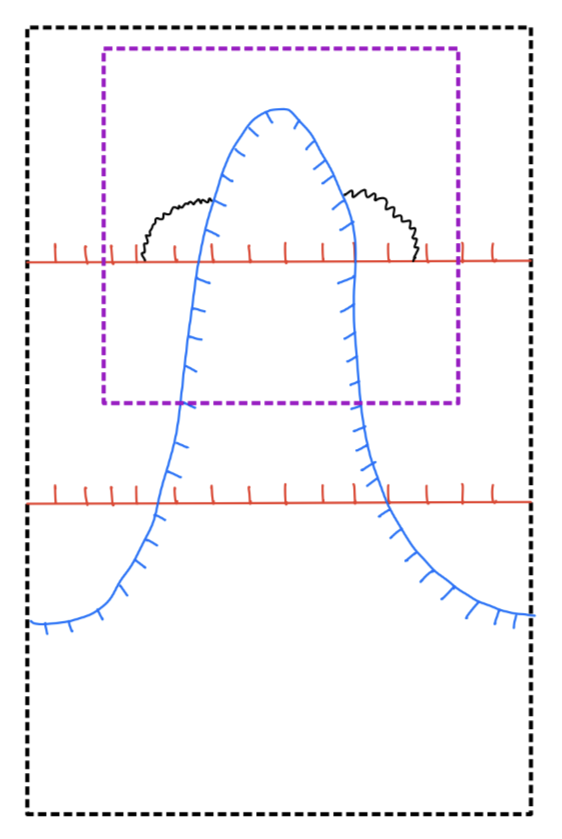
\includegraphics[width=\linewidth]{diagrams/lemma8/3.png} % Adjust the width as needed
    \caption{Your caption here}
    \label{fig:your-label}
\end{figure}

We get the following diagram :

\begin{figure}[H] % Optional: [h] means here, [t] for top, [b] for bottom, [p] for page of floats
    \centering
    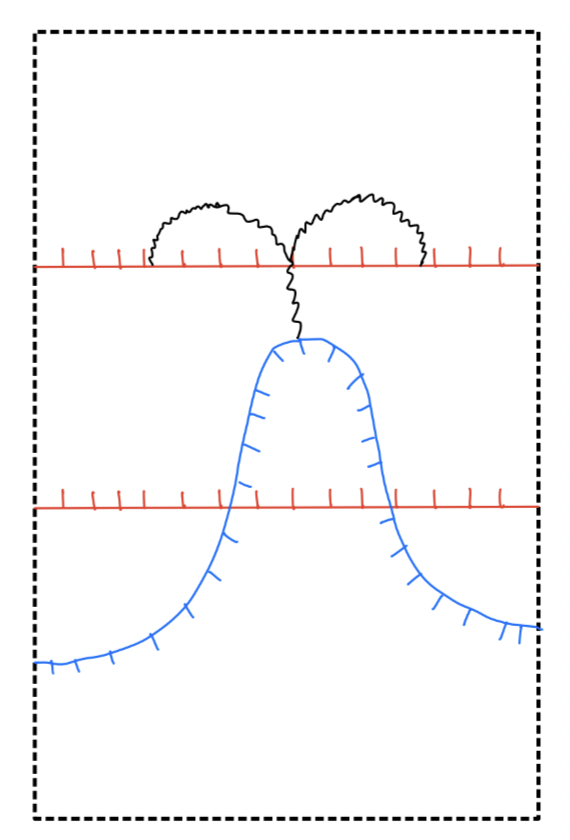
\includegraphics[width=\linewidth]{diagrams/lemma8/4.png} % Adjust the width as needed
    \caption{Your caption here}
    \label{fig:your-label}
\end{figure}

(step2) Apply $isotopy_5$ on the disk surrounded by the purple dotted line:
\begin{figure}[H] % Optional: [h] means here, [t] for top, [b] for bottom, [p] for page of floats
    \centering
    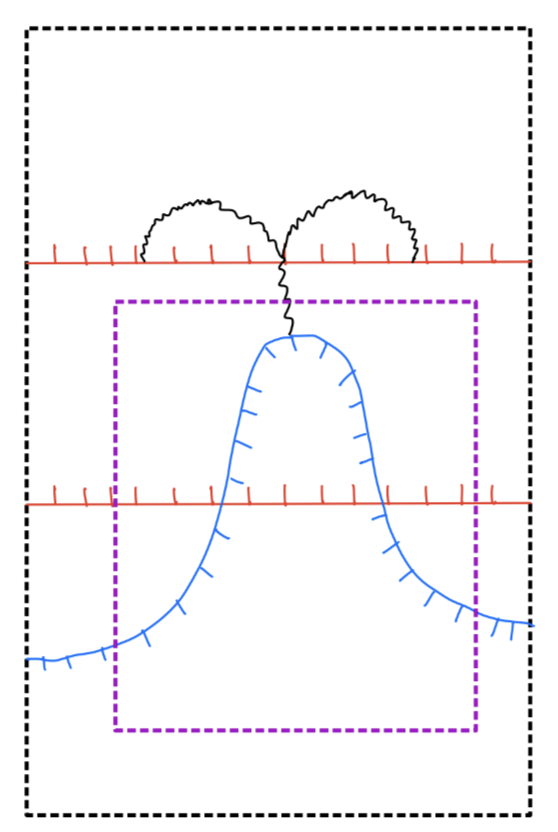
\includegraphics[width=\linewidth]{diagrams/lemma8/5.png} % Adjust the width as needed
    \caption{Your caption here}
    \label{fig:your-label}
\end{figure}

We get the final diagram :

\begin{figure}[H] % Optional: [h] means here, [t] for top, [b] for bottom, [p] for page of floats
    \centering
    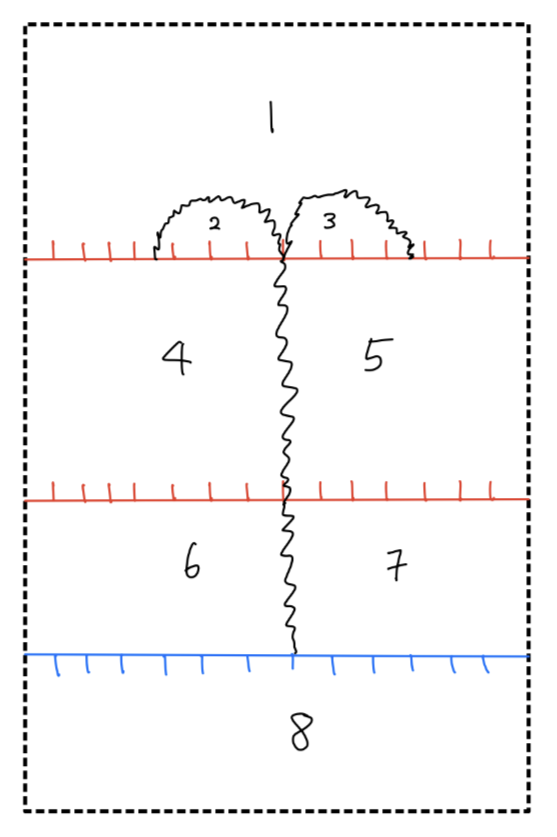
\includegraphics[width=\linewidth]{diagrams/lemma8/2.png} % Adjust the width as needed
    \caption{Your caption here}
    \label{fig:your-label}
\end{figure}

with sheaf $\mathfrak{F}'$ on it.\\
(proof)